\documentclass[12pt]{article}

% Layout.
\usepackage[top=1.2in, bottom=0.75in, left=1in, right=1in, headheight=1.0in, headsep=0pt]{geometry}

% Fonts.
\usepackage{mathptmx}
\usepackage[scaled=0.86]{helvet}
\renewcommand{\emph}[1]{\textsf{\textbf{#1}}}

% TiKZ.
\usepackage{tikz, pgfplots}
\usetikzlibrary{calc}
\pgfplotsset{my style/.append style={axis x line=middle, axis y line=middle, xlabel={$x$}, ylabel={$y$}}}
\pgfplotsset{compat=1.18}

% Misc packages.
\usepackage{amsmath,amssymb,latexsym}
\usepackage{graphicx}
\usepackage{array}
\usepackage{xcolor}
\usepackage{multicol}

% Commands to set various header/footer components.
\makeatletter
\def\doctitle#1{\gdef\@doctitle{#1}}
\doctitle{Use {\tt\textbackslash doctitle\{MY LABEL\}}.}
\def\docdate#1{\gdef\@docdate{#1}}
\docdate{Use {\tt\textbackslash docdate\{MY DATE\}}.}
\def\doccourse#1{\gdef\@doccourse{#1}}
\let\@doccourse\@empty
\def\docscoring#1{\gdef\@docscoring{#1}}
\let\@docscoring\@empty
\def\docversion#1{\gdef\@docversion{#1}}
\let\@docversion\@empty
\makeatother

% Headers and footers layout.
\makeatletter
\usepackage{fancyhdr}
\pagestyle{fancy}
\fancyhf{} % Clears all headers/footers.
\lhead{\emph{\@doctitle\hfill\@docdate} \medskip
\ifnum \value{page} > 1\relax\else\\
\emph{Name: \rule{3.5in}{1pt}\hfill \@docscoring}
\fi}

\rfoot{\emph{\@docversion}}
\lfoot{\emph{\@doccourse}}
\cfoot{\emph{\thepage}}
\renewcommand{\headrulewidth}{0pt}%
\makeatother

% Paragraph spacing
\parindent 0pt
\parskip 6pt plus 1pt

% A problem is a section-like command. Use \problem{5} for a problem worth 5 points.
\newcounter{probcount}
\newcounter{subprobcount}
\setcounter{probcount}{0}

\newcommand{\problem}[1]{%
\par
\addvspace{4pt}%
\setcounter{subprobcount}{0}%
\stepcounter{probcount}%
\makebox[0pt][r]{\emph{\arabic{probcount}.}\hskip1ex}\emph{[#1 points]}\hskip1ex}

\newcommand{\thesubproblem}{\emph{\alph{subprobcount}.}}

% like \problem but with name
\newcommand{\nameprob}[2]{%
\par
\addvspace{4pt}%
\setcounter{subprobcount}{0}%
\stepcounter{probcount}%
\makebox[0pt][r]{\emph{#1.}\hskip1ex}\emph{[#2 points]}\hskip1ex}

% Subproblems are an enumerate-like environment with a consistent
% numbering scheme.  Use \begin{subproblems}\item...\item...\end{subproblems}
\newenvironment{subproblems}{%
\begin{enumerate}%
\setcounter{enumi}{\value{subprobcount}}%
\renewcommand{\theenumi}{\emph{\alph{enumi}}}}%
{\setcounter{subprobcount}{\value{enumi}}\end{enumerate}}

% Blanks for answers in normal and math mode.
\newcommand{\blank}[1]{\rule{#1}{0.75pt}}
\newcommand{\mblank}[1]{\underline{\hspace{#1}}}
\def\emptybox(#1,#2){\framebox{\parbox[c][#2]{#1}{\rule{0pt}{0pt}}}}

% Misc.
\renewcommand{\d}{\displaystyle}
\newcommand{\ds}{\displaystyle}


\doctitle{Math 252: Quiz 3 }
\docdate{11 Sept 2025}
\doccourse{}
\docversion{}
\docscoring{\fbox{{\LARGE \strut}\blank{0.8in} / 25}}

\begin{document}
30 minutes maximum.  No aids (book, calculator, etc.) are permitted.  Show all work and use proper notation for full credit.  Answers should be in reasonably-simplified form.  25 points possible.

\begin{enumerate}
% [Like 2.3 #114,120,122] 
\item (9 points) The region $R$ is bounded by $y=\sqrt{1+2x^2},$ $x=2$, and the $x$- and $y$- axes. Sketch the region $R$ on the graph below and answer the questions. \\
%%%% GRAPH OF R
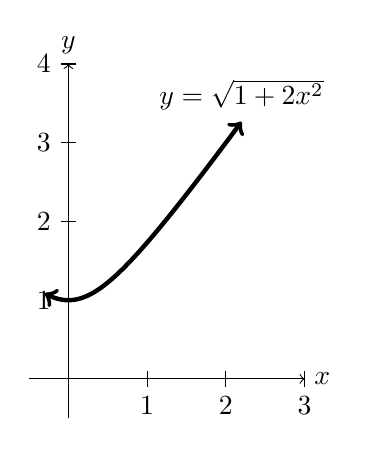
\begin{tikzpicture}[scale=1, yscale=1]
    % Define the coordinate system
    \draw[->] (-0.5,0) -- (3,0) node[right] {$x$};
    \draw[->] (0,-0.5) -- (0,4) node[above] {$y$};
    
       % Axis labels
    \foreach \x in {1,2,3}
        \draw (\x,0.1) -- (\x,-0.1) node[below] {$\x$};
    \foreach \y in {1,2,3,4}
        \draw (0.1,\y) -- (-0.1,\y) node[left] {$\y$};
    
    % Plot y = f(x)
    \draw[domain=-0.3:2.2, samples=100, ultra thick, black,<->] 
        plot (\x,{(1+\x*\x*2)^(0.5)}) node[above] {$y = \sqrt{1+2x^2}$};
    
\end{tikzpicture}
%%% End of graph

	\begin{enumerate}
	\item (7 points) \textbf{Use shells} to find the volume of the solid obtained by rotating the region $R$ about the \fbox{$y$-axis}. (You must \textbf{set-up} an integral and \textbf{evaluate} it.)\\
	\vfill
	
	\vfill
	
	\item (2 points) Give at least one reason why the method of shells might be better than disks or washers for the problem in part (a).\\	
	\vspace{.5in}
	
	\end{enumerate}
\newpage
%[2.3 # 132, 138]	
\item (5 points)  Suppose the region $R$ is bounded by  $y=3x^{2/3}$, $y=\frac{4}{x} -1$ and the $x$-axis. (Graphed below.) \textbf{Set up but do not evaluate} an integral for finding the volume of the solid generated by rotating $R$ about the \fbox{$x$-axis}. \textbf{Use shells.}\\

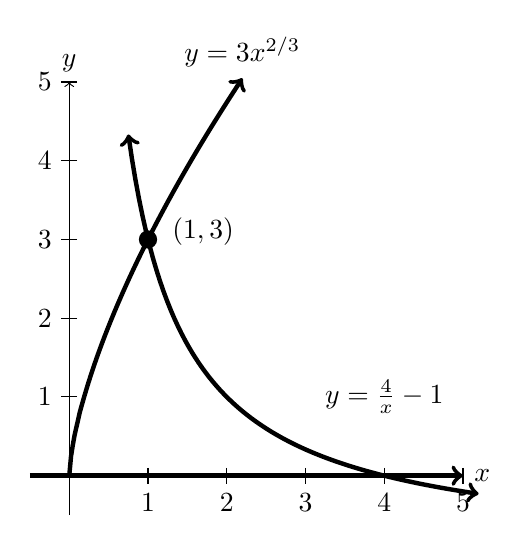
\begin{tikzpicture}[scale=1, yscale=1]
    % Define the coordinate system
    \draw[->, ultra thick ] (-0.5,0) -- (5,0) node[right] {$x$};
    \draw[->] (0,-0.5) -- (0,5) node[above] {$y$};
    
       % Axis labels
    \foreach \x in {1,2,3,4,5}
        \draw (\x,0.1) -- (\x,-0.1) node[below] {$\x$};
    \foreach \y in {1,2,3,4,5}
        \draw (0.1,\y) -- (-0.1,\y) node[left] {$\y$};
    
    % Plot rhs
    \draw[domain=0:2.2, samples=100, ultra thick, black,->] 
        plot (\x,{3*(\x)^(0.66)}) node[above] {$y = 3x^{2/3}$};
    \draw[domain=0.75:5.2, samples=100, ultra thick, black,<->] 
        plot (\x,{(4/ \x) -1});
    \node at (4,1) {$y = \frac{4}{x}-1$};
    
    %add point
    \node[black, circle, fill, scale=.7] at (1,3){};
    \node at (1.7,3.1){$(1,3)$};
    
\end{tikzpicture}
%%% End of graph

Formulas: \hspace{.3in} $\text{arc length} = \displaystyle{\int_a^b}\sqrt{1+(f'(x))^2} \: dx$ \hspace{.3in} $\text{surface area} = \displaystyle{\int_a^b}2 \pi f(x)\sqrt{1+(f'(x))^2} \: dx$
% [like 2.2 \# 76-98]
\item (3 points)  \textbf{Set up but do not evaluate} an integral to calculate the length of the function $y=\ln(x^2+1)$ from $x=0$ to $x=10.$

\vfill

\item (8 points) Find the surface area of the volume generated when the curve $f(x)=\sqrt{4-x^2}$ from $x=0$ to $x=1$ is revolved around the $x$-axis. (You can evaluate this integral. The points will be distributed as: 5 points to correctly set up the integral and 3 points for the work to correctly evaluate it.)

\vfill

\vfill

\vfill
 


\end{enumerate}
\end{document}

